\title{Kepler's Laws of Planetary Motion}
\author{Dr. Jordan Hanson - Whittier College Dept. of Physics and Astronomy}
\date{\today}
\documentclass[12pt]{article}
\usepackage[margin=1.25cm]{geometry}
\usepackage{hyperref}
\usepackage{graphicx}
\usepackage{amsmath}
\usepackage{subcaption}
\begin{document}
\twocolumn
\maketitle

\begin{figure}
\centering
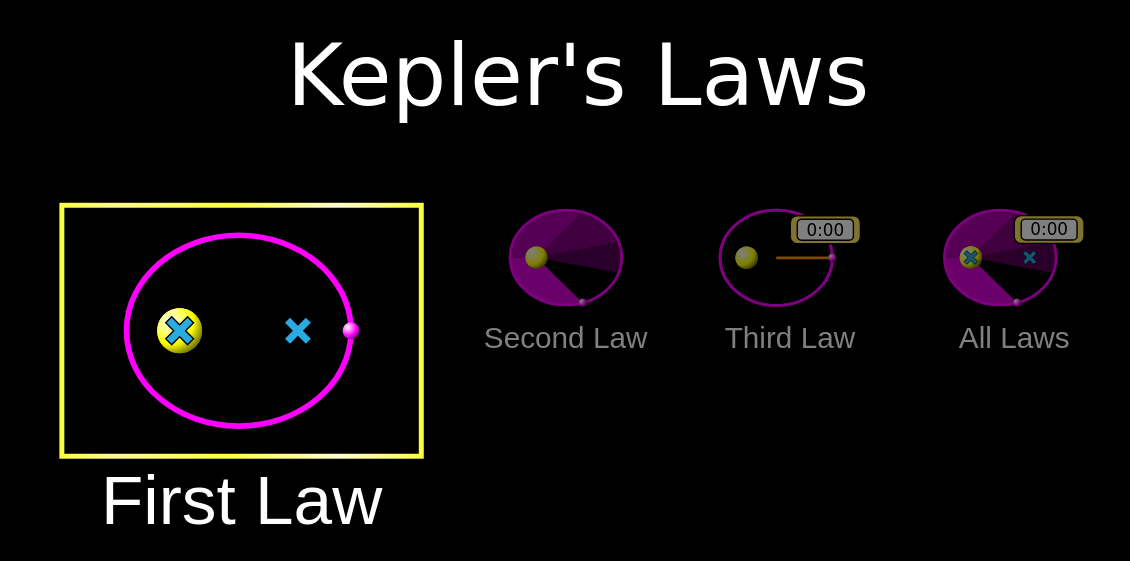
\includegraphics[width=0.45\textwidth]{figures/kepler3.png}
\caption{\label{fig:1b} PhET simulation for Kepler's Laws.}
\end{figure}

\section{Introduction}

In this simulation activity, we will explore Kepler's laws.  We will derive Kepler's 3rd law using centripetal force and the force of gravity, explore the orbital parameter space, and graph orbital period versus orbital radius.

\section{Kepler's First and Second \\ Laws}

Kepler's First and Second Laws: \textit{The orbit of a planet is an ellipse with the Sun at one of the two foci,} and \textit{a line segment joining a planet and the Sun sweeps out equal areas during equal intervals of time}.  (a) Open the First Law tab in the simulation, and set the target orbit to Venus.  (b) Arrange the velocity and position of the planet so that the orbit matches that of Venus. Click play.  (c) Now set the target orbit to that of the Earth.  (d) Why are we (rarely) able to observe Venus transit across the face of the Sun, from our perspective? (e) Open the Second Law tab in the simulation, and set the period divisions to 6.  Check the area and time boxes and click play.  (f) Is swept area per unit time constant? \\ \vspace{2cm}

\section{Kepler's Third Law}

Kepler's 3rd law states that \textit{the square of a planet's orbital period is proportional to the cube of the length of the semi-major axis of its orbit.}
\begin{itemize}
\item To orbit a star, a planet must experience a force that provides centripetal acceleration.  The force of gravity between Sun and planet provides this, and we will work with a circular orbit approximation to prove Kepler's 3rd law.  Let $G = 6.67\times 10^{-11}$ N m$^2$ kg$^{-2}$.  Further, let $M$ be the mass of the Sun, $m$ be the mass of the planet, $r$ be the orbital radius, $\omega$ be the angular velocity, and $T$ be the orbital period.  The force of gravity and centripetal force are
\begin{align}
\vec{F}_{\rm G} &= G\frac{Mm}{r^2}\hat{r} \label{eq:1} \\
\vec{F}_{\rm C} &= -m\vec{r}\omega^2 \label{eq:2} 
\end{align}
If the force of gravity does not equal the centripetal force, the orbital radius will change until they are equal.  (a) Set Eq. \ref{eq:1} and \ref{eq:2} equal, and solve for $r^3$. (b) Note that $\omega$ is the angular velocity, so for one period, $\omega = 2\pi/T$.  Substitute this idea into your equation, and obtain a formula involving $r^3$ and $T^2$.
\item Using a variety of orbital radii, velocities, and periods, collect enough data to plot $T^2$ vs. $r^3$.  Fit your formula relating $T^2$ and $r^3$ to the simulation data.  Note that the fit works even for elliptical (non-circular) orbits.  We will address the proof of this in Chapter 13.
\end{itemize}
\end{document}
